\documentclass[ngerman]{gdb-aufgabenblatt}
\RequirePackage[utf8]{inputenc}
\renewcommand{\Aufgabenblatt}{6}
\renewcommand{\Ausgabedatum}{Mi. 08.01.2014}
\renewcommand{\Abgabedatum}{Do. 23.01.2014}
\renewcommand{\Gruppe}{Tim Dittrich, Sebastian Lindemann, Jim Martens}

% define how the sections are rendered
\def\thesection{Aufgabe \arabic{section}:}
\def\thesubsection{\alph{subsection})}
\def\thesubsubsection{\roman{subsubsection})}

\usetikzlibrary{positioning}
\usetikzlibrary{shadows}

\begin{document}
\section{B-Bäume}
	\subsection{} %a
		42 kann einfach eingefügt werden. Zum Einfügen von 6 wird der Baum gesplittet. Damit ergibt sich dieser Baum:
		
		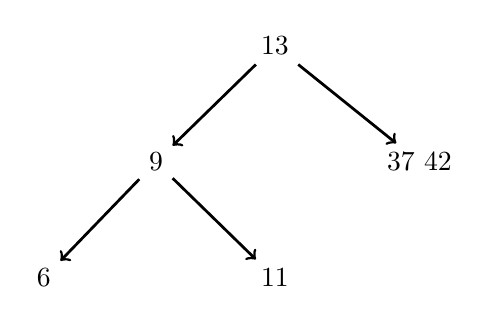
\begin{tikzpicture}
			\node (root) {13};
			\node (1-l) [below left=of root] {9};
			\node (1-r) [below right=of root] {37 42};
			\node (2-l) [below left=of 1-l] {6};
			\node (2-r) [below right=of 1-l] {11};
			\path[->,line width=1pt] 
			    (root) edge (1-l)
			    (root) edge (1-r)
			    (1-l) edge (2-l)
			    (1-l) edge (2-r);
		\end{tikzpicture}
		
		12 kann wieder einfach eingefügt werden. Bei 25 muss der Baum wieder gesplittet werden, womit sich dieser Baum ergibt:
		
		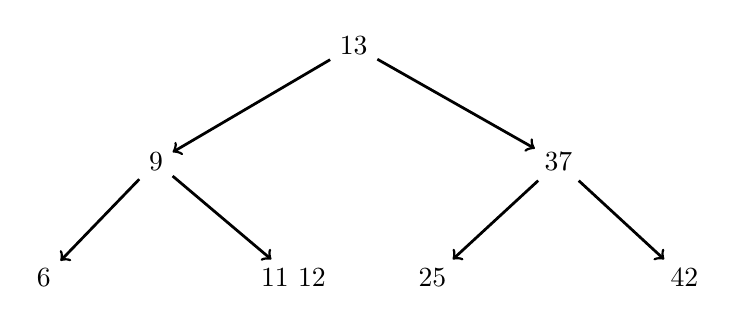
\begin{tikzpicture}
			\node (root) {13};
			\node (1-l) [below left=1 and 2 of root] {9};
			\node (1-r) [below right=1 and 2 of root] {37};
			\node (2-l) [below left=of 1-l] {6};
			\node (2-r) [below right=of 1-l] {11 12};
			\node (2-rl) [below left=of 1-r] {25};
			\node (2-rr) [below right=of 1-r] {42};
			\path[->,line width=1pt] 
			    (root) edge (1-l)
			    (root) edge (1-r)
			    (1-l) edge (2-l)
			    (1-l) edge (2-r)
			    (1-r) edge (2-rl)
			    (1-r) edge (2-rr);
		\end{tikzpicture}
	\subsection{} %b
		Für das Löschen von 17 wird der Baum ausgeglichen. Es ergibt sich dieser Baum:
		
		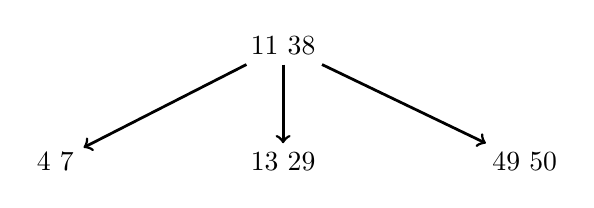
\begin{tikzpicture}
			\node (root) {11 38};
			\node (1-l) [below left=1 and 2 of root] {4 7};
			\node (1-m) [below=of root] {13 29};
			\node (1-r) [below right=1 and 2 of root] {49 50};
			\path[->,line width=1pt] 
			    (root) edge (1-l)
			    (root) edge (1-r)
			    (root) edge (1-m);
		\end{tikzpicture}
		
		29 kann mit Mischen gelöscht werden. Es ergibt sich dieser Baum:
		
		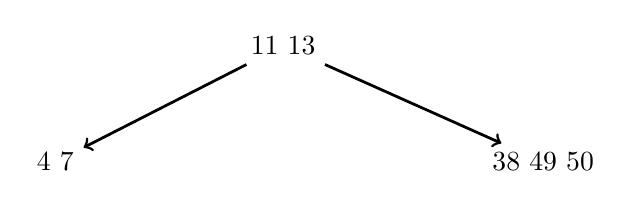
\begin{tikzpicture}
			\node (root) {11 13};
			\node (1-l) [below left=1 and 2 of root] {4 7};
			\node (1-r) [below right=1 and 2 of root] {38 49 50};
			\path[->,line width=1pt] 
			    (root) edge (1-l)
			    (root) edge (1-r);
		\end{tikzpicture}
		
		49 kann einfach gelöscht werden. 7 kann nicht mehr gelöscht werden, ohne die Bedingungen eines B-Baumes zu verletzen. Nach dem Löschen von 7 blieben noch 5 Schlüssel übrig. Da pro Knoten mindestens 2 und maximal 4 Schlüssel eingetragen sein dürfen, wäre die einzige Lösung einen Knoten mit 2 und einen mit 3 Einträgen zu haben. Dies widerspräche aber der Voraussetzung, dass die Wurzel mindestens 2 Söhne hat, sofern sie kein Blatt ist. Daher ist diese Operation nicht möglich.
		
		Wenn jedoch 7 und 4 zusammen gelöscht würden, dann ergäbe sich dieser Baum:
		
		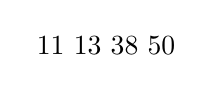
\begin{tikzpicture}
			\node (root) {11 13 38 50};
		\end{tikzpicture}
\section{Berechnungen in B-Bäumen}
	\subsection{} %a
		\subsubsection{} %i
			Der Baum kann minimal 6 Einträge und maximal 24 Einträge haben.
		\subsubsection{} %ii
			\[
				\frac{z_{max}}{n_{max}}
			\]
	\subsection{} %b
		\subsubsection{} %i
			maximale Belegung von Bäumen der angegebenen Klasse nach Höhe:
			
			\begin{itemize}
				\item h=1: 6
				\item h=2: 48
				\item h=3: 348
			\end{itemize}
			
			Demnach muss der B-Baum mindestens eine Höhe von 3 haben, um alle Datensätze fassen zu können.
		\subsubsection{} %ii
		
			minimale Belegung von Bäumen der angegebenen Klasse nach Höhe:
			
			\begin{itemize}
				\item h=1: 3
				\item h=2: 9
				\item h=3: 33
				\item h=4: 141
			\end{itemize}
			
			Demnach kann der B-Baum maximal eine Höhe von 4 haben, um alle Datensätze fassen zu können.
\section{B*-Bäume}
	\subsection{} %a
		64 kann einfach eingefügt werden. Beim Einfügen von 3 wird gesplittet:
		
		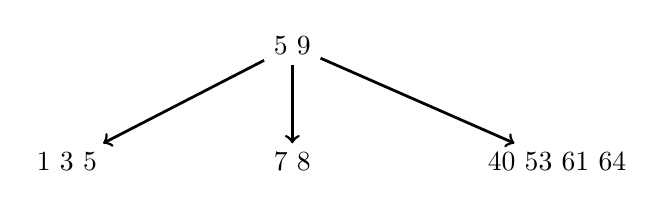
\begin{tikzpicture}
			\node (root) {5 9};
			\node (1-l) [below left=1 and 2 of root] {1 3 5};
			\node (1-m) [below=of root] {7 8};
			\node (1-r) [below right=1 and 2 of root] {40 53 61 64};
			
			\path[->,line width=1pt] (root) edge (1-l)
				(root) edge (1-m)
				(root) edge (1-r);
		\end{tikzpicture}
		
		6 kann einfach eingefügt werden. Beim Einfügen von 80 wird gesplittet:
		
		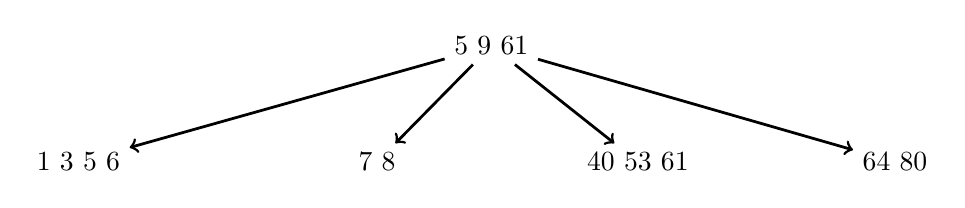
\begin{tikzpicture}
			\node (root) {5 9 61};
			\node (1-l) [below left=1 and 4 of root] {1 3 5 6};
			\node (1-ml) [below left=1 and 0.5 of root] {7 8};
			\node (1-mr) [below right=1 and 0.5 of root] {40 53 61};
			\node (1-r) [below right=1 and 4 of root] {64 80};
			
			\path[->,line width=1pt] (root) edge (1-l)
				(root) edge (1-ml)
				(root) edge (1-mr)
				(root) edge (1-r);
		\end{tikzpicture}
	\subsection{} %b
		14 wird einfach gelöscht.
		
		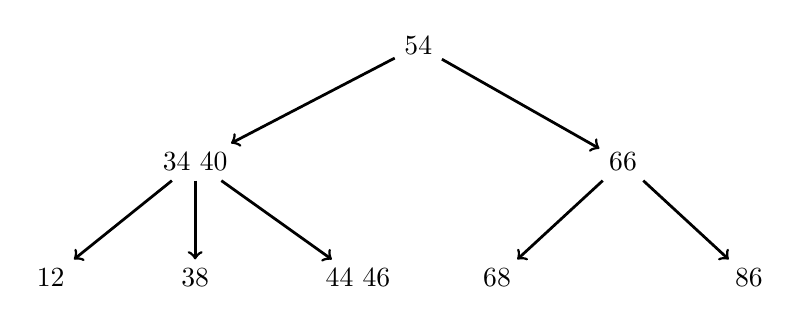
\begin{tikzpicture}
			\node (root) {54};
			\node (1-l) [below left=1 and 2 of root] {34 40};
			\node (1-r) [below right=1 and 2 of root] {66};
			\node (2-ll) [below left=1 and 1 of 1-l] {12};
			\node (2-lm) [below=of 1-l] {38};
			\node (2-lr) [below right=1 and 1 of 1-l] {44 46};
			\node (2-rl) [below left=1 and 1 of 1-r] {68};
			\node (2-rr) [below right=1 and 1 of 1-r] {86};
			\path[->,line width=1pt] (root) edge (1-l)
				(root) edge (1-r)
				(1-l) edge (2-ll)
				(1-l) edge (2-lm)
				(1-l) edge (2-lr)
				(1-r) edge (2-rl)
				(1-r) edge (2-rr);
		\end{tikzpicture}
		
		38 kann einfach gelöscht werden.
		
		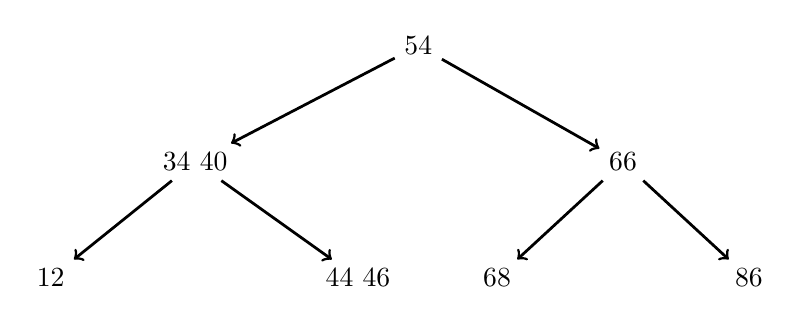
\begin{tikzpicture}
			\node (root) {54};
			\node (1-l) [below left=1 and 2 of root] {34 40};
			\node (1-r) [below right=1 and 2 of root] {66};
			\node (2-ll) [below left=1 and 1 of 1-l] {12};
			\node (2-lr) [below right=1 and 1 of 1-l] {44 46};
			\node (2-rl) [below left=1 and 1 of 1-r] {68};
			\node (2-rr) [below right=1 and 1 of 1-r] {86};
			\path[->,line width=1pt] (root) edge (1-l)
				(root) edge (1-r)
				(1-l) edge (2-ll)
				(1-l) edge (2-lr)
				(1-r) edge (2-rl)
				(1-r) edge (2-rr);
		\end{tikzpicture}
		
		12 kann durch Mischen gelöscht werden.
		
		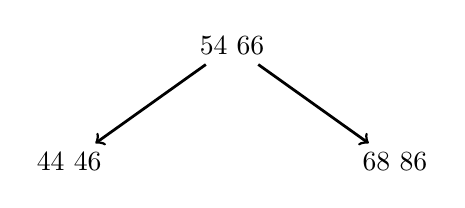
\begin{tikzpicture}
			\node (root) {54 66};
			\node (1-l) [below left=1 and 1 of root] {44 46};
			\node (1-r) [below right=1 and 1 of root] {68 86};
			\path[->,line width=1pt] (root) edge (1-l)
				(root) edge (1-r);
		\end{tikzpicture}
		
		44 kann einfach gelöscht werden.
		
		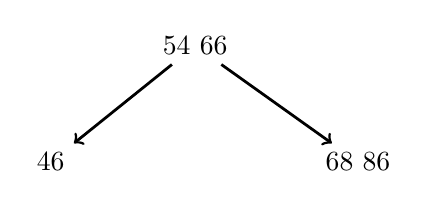
\begin{tikzpicture}
			\node (root) {54 66};
			\node (1-l) [below left=1 and 1 of root] {46};
			\node (1-r) [below right=1 and 1 of root] {68 86};
			\path[->,line width=1pt] (root) edge (1-l)
				(root) edge (1-r);
		\end{tikzpicture}
\section{Normalformenlehre}
	\subsubsection{} %i
		Die Schlüsselkanidaten von R bezüglich F sind B und A,D.
	\subsubsection{} %ii
		Die Nicht-Primärattribute von R bezüglich F sind E und C.
	\subsubsection{} %iii
		C hängt partiell von A,D ab, aber nicht von B. Daher befindet sich die Relation nicht in der zweiten Normalform und damit auch nicht in der dritten. Da jedes der Attribute in R atomar ist, befindet sich R in der ersten Normalform.
\end{document}